\documentclass{article}

% De esta forma se pueden usar caracteres del UTF-8
\usepackage[utf8]{inputenc}
\usepackage{listings}
\usepackage{color}
\usepackage{graphicx}

\definecolor{dkgreen}{rgb}{0,0.6,0}
\definecolor{gray}{rgb}{0.5,0.5,0.5}
\definecolor{mauve}{rgb}{0.58,0,0.82}

\lstset{frame=tb,
  language=C++,
  aboveskip=3mm,
  belowskip=3mm,
  showstringspaces=false,
  columns=flexible,
  basicstyle={\small\ttfamily},
  numbers=none,
  numberstyle=\tiny\color{gray},
  keywordstyle=\color{blue},
  commentstyle=\color{dkgreen},
  stringstyle=\color{mauve},
  breaklines=true,
  breakatwhitespace=true,
  tabsize=4
}

% De esta forma se establece el titulo (esta zona es el preambulo)
\title{
	MEMORIA: EJERCICIO DE SUMA DE SUBCONJUNTOS \\ % \\ termina la linea
	\large Estudio empírico de la eficiencia \\
	con el uso de distintas estrategias}
\author{Vladislav Nikolov Vasilev, 2ºA}



\begin{document}
  \pagenumbering{gobble} % Con esto se oculta el numero de pagina
  \maketitle			  % Se inserta el titulo creado en el preambulo
  \newpage				  % Se inserta una nueva pagina
  \pagenumbering{arabic} % Se utiliza la numeracion de pagina arabica
  
  \section{Introducción}
  En este ejercicio se ha pedido que se implementen tres versiones de un programa que, dado un conjunto de \textit{n} números que van desde 1 hasta \textit{n}+1, y un número \textit{M}, encuentre todos los subconjuntos de números que sumen exactamente \textit{M}. Adicionalmente se ha pedido realizar un análisis empírico con las tres versiones para ver cuál de ellas era la más eficiente respecto al tiempo que tardaba en realizar los cálculos.\\\\
  En esta memoria se va a realizar primero una explicación rápida de la implementación realizada en cada una de las versiones, y a continuación se mostrarán los resultados del estudio empírico realizado para determinar cuál es la implementación más eficiente.
  
  \section{Implementación}
  En general, para todas las implementaciones realizadas, se ha utilizado el TDA \textbf{Solucion} que aparecía en las transparencias de clase, modificándolo según las necesidades de la versión. En casi todas las versiones se han implementado los métodos de la misma forma que estaban especificados en las transparencias, excepto en las que se comentarán más abajo. Adicionalmente se ha implementado un método extra para una de las versiones que permita comprobar que los resultados obtenidos son los correctos. Cabe mencionar además que se ha incluido un atributo más al TDA, \textit{objetivo}, que se corresponde con el número \textit{M} mencionado anteriormente, y que los números que conforman el vector \textit{w} han sido inicializados desde 1 hasta \textit{n}+1, siendo \textit{n} el tamaño del vector solución.\\\\
  La primera versión ha consistido en la implementación de un algoritmo de \textit{fuerza bruta} que se ha encargado de construir todos los posibles subconjuntos de números. Para ello, se ha hecho uso de una función recursiva que ha permitido recorrer el árbol de estados generando los correspondientes nodos sucesores. En este caso se ha implementado un método adicional que recorre el vector solución y comprueba si se da que:
  \[
  \sum_{i=0}^{n}X[i]w[i]=M
  \]
  A continuación se adjunta el código de la función recursiva:
  \begin{lstlisting}
  void fuerzaBruta(Solucion& sol, int k) {
    if (k == sol.size()) {
        if (sol.solucionCorrecta()) {
            sol.procesaSolucion();
        }
    } else {
        sol.iniciaComp(k);
        sol.sigValComp(k);

        while (!sol.todosGenerados(k)) {
            fuerzaBruta(sol, k + 1);
            sol.sigValComp(k);
        }
    }
  }
  \end{lstlisting} 
  En la segunda versión implementada se ha utilizado una estrategia de backtracking que no guarda la información que se va obteniendo para cada decisón. Esto implica que para cada decisón tomada se tiene que utilizar un tiempo extra, que en el peor de los casos es $\mathcal{O}(n)$, para calcular la factibilidad de esa solución, ya que se tiene que recorrer el conjunto elementos que conforman la solución parcial y de las soluciones restantes y realizar los cálculos necesarios. En este caso también se ha utilizado una función recursiva para recorrer el árbol de estados, y el código implementado se deja a continuación:
  \begin{lstlisting}
  void backRecursivo(Solucion& sol, int k) {
    if (k == sol.size()) {
        sol.procesaSolucion();
    } else {
        sol.iniciaComp(k);
        sol.sigValComp(k);

        while (!sol.todosGenerados(k)) {
            if (sol.factible(k))
                backRecursivo(sol, k + 1);
            sol.sigValComp(k);
        }
    }
  }
  \end{lstlisting}
  La tercera versión que se ha implementado es una variación de la anterior. En este caso también se ha utilizado una estrategia de backtracking, solo que en este caso en el momento en el que se elige o quita un número de la solución parcial se realizan las cuentas necesarias para que luego al comprobar la factibilidad de la solución se consiga hacer en $\mathcal{O}(1)$. En esta tercera versión también se ha utilizado una función recursiva para recorrer el árbol de estados, además de crear un nuevo método que permita deshacer el camino tomado cuando se realiza el backtracking. El código de esa función es el siguiente:
  \begin{lstlisting}
  void backRecursivo(Solucion& sol, int k) {
    if (k == sol.size()) {
        sol.procesaSolucion();
    } else {
        sol.iniciaComp(k);
        sol.sigValComp(k);

        while (!sol.todosGenerados(k)) {
            if (sol.factible(k)) {
                backRecursivo(sol, k + 1);
                sol.vueltaAtras(k + 1);
            }
            sol.sigValComp(k);
        }
    }
  }
  \end{lstlisting}
  
  \section{Análisis de eficiencia empírica}
  A la hora de realizar el análisis se han ejecutado las tres versiones con un tamaño que estaba comprendido en el intervalo [5, 28], ya que el tiempo del algoritmo de fuerza bruta se disparaba demasiado rápido a medida que aumentaba el tamaño, y se ha pedido que se busquen todos los números que sumasen \textit{tam}+1. Los resultados que se han obtenido para las tres versiones son los siguientes:
  \begin{center}
  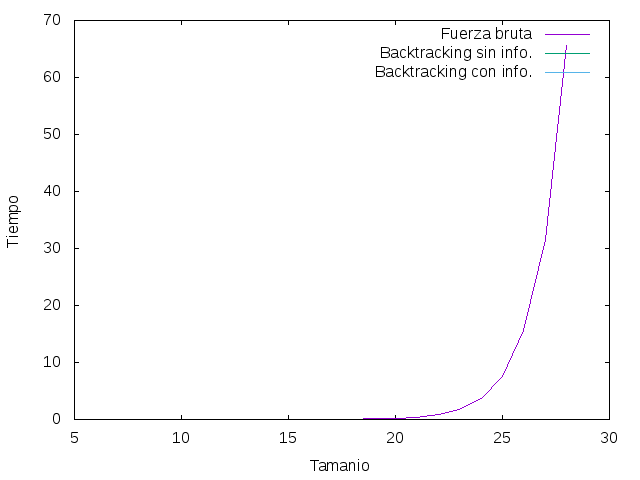
\includegraphics[scale=0.70]{screenshots/comparacion_3.png}
  \end{center}
  Como se puede comprobar a simple vista, los tiempos que ofrece la versión de fuerza bruta son pésimos, ya que para tamaños relativamente pequeños, como es el caso de 28, tarda aproximadamente 70 segundos en encontrar todas las soluciones. Además, como los tiempos de las dos versiones del backtracking son muy pequeños no se ven bien, y por tanto se proceden a mostrar a continuación:
  \begin{center}
  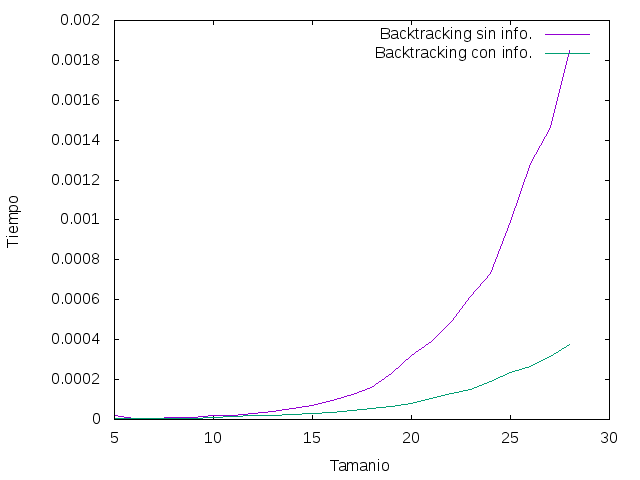
\includegraphics[scale=0.70]{screenshots/comparacion_back_28.png}
  \end{center}
  Aquí se puede ver claramente como la versión de backtracking con información ofrece unos tiempos muchísimo mejores que la versión sin información. Esta segunda, a pesar de ser peor que la versión con información, es infinitamente mejor que la versión de fuerza bruta.\\\\
  Adicionalmente, para las versiones de backtracking se ha seguido comprobando para tamaños mayores qué tiempos se obtienen, llegando a probar hasta un tamaño de 50. Los resultados obtenidos son los siguientes:
  \begin{center}
  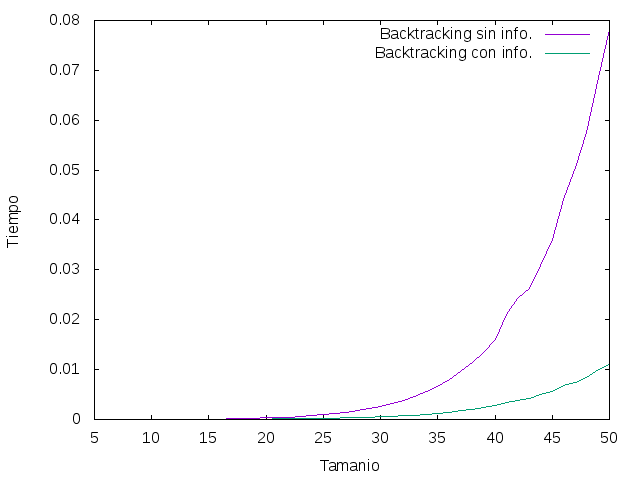
\includegraphics[scale=0.70]{screenshots/comparacion_back_50.png}
  \end{center}
  De aquí se puede concluir que, la versión de fuerza bruta es la peor de las tres, la versión de backtracking sin información es una aproximación muy buena para resolver el problema en un tiempo aceptable, pero que lo más idóneo es utilizar una versión de backtracking con información, ya que la comprobación de factibilidad pasa de ser $\mathcal{O}(n)$ a $\mathcal{O}(1)$, reduciendo drásticamente los tiempos de ejecución.
  
\end{document}